\documentclass[preprint,12pt,a4paper]{elsarticle}
\pdfinfoomitdate=1\pdftrailerid{}
\usepackage{amssymb,amsmath,booktabs,array,float,hyperref,xurl,placeins}
\newcolumntype{P}[1]{>{\raggedright\arraybackslash}p{#1}}
\setlength{\parindent}{0pt}\setlength{\emergencystretch}{1.5em}
\clubpenalty=10000\widowpenalty=10000
\setlength{\abovecaptionskip}{6pt}\setlength{\belowcaptionskip}{4pt}
\setlength{\textfloatsep}{14pt plus 2pt minus 2pt}
\hypersetup{hidelinks}\journal{SoftwareX}
\renewcommand{\topfraction}{.9}\renewcommand{\textfraction}{.05}\renewcommand{\floatpagefraction}{.8}
\renewcommand{\bibfont}{\footnotesize}
\setlength{\bibsep}{0pt}
\begin{document}\begin{frontmatter}
\title{WorkCert: Reconstruction error metadata for force--displacement tables}
\author[a]{Saisai Hou}\author[a]{Yunzhi Zhu}\author[a]{Sen Zhang\corref{cor}}
\cortext[cor]{Corresponding author.}\ead{szhang@niit.edu.cn}
\affiliation[a]{organization={Department of Public Basic Courses, Nanjing University of Industry Technology},city={Nanjing},country={China}}
\begin{abstract}
WorkCert is a Python package for reduced force--displacement tables that carry reconstruction-error metadata and support reusable work queries. Its interface combines established simplification and integration methods with source verification, serialization and chronological branch handling. Public-data examples demonstrate energy-absorption screening, selective refinement and work-to-stroke inversion. A checked cyclic workflow rejects unmet branch budgets and requests targeted refinement. Across 70 references, changing the stopping measure within the same work-priority selector reduces median table size from 27 to 14 nodes for a 1\% interval-work requirement. The errors describe reconstruction of the supplied numerical reference and exclude measurement uncertainty and floating-point rounding. Code, data and reproducible evaluation scripts accompany the software.
\end{abstract}
\begin{keyword}Research software\sep Force--displacement data\sep Reconstruction error\sep Energy absorption\sep Stable integration\sep Cyclic response\end{keyword}
\end{frontmatter}\clearpage
\section*{Required Metadata}\section*{Current code version}
\begin{table}[H]\small\centering
\begin{tabular}{|P{.05\linewidth}|P{.39\linewidth}|P{.425\linewidth}|}\hline
\textbf{Nr.}&\textbf{Code metadata description}&\textbf{Metadata}\\\hline
C1&Current code version&0.3.0\\\hline
C2&Permanent GitHub link to code/repository used for this code version&\url{https://github.com/changs1723/WorkCert/tree/v0.3.0}\\\hline
C3&Legal Code License&MIT License\\\hline
C4&Code versioning system used&Git\\\hline
C5&Software code languages, tools, and services used&Python; NumPy; command-line interface\\\hline
C6&Compilation requirements, operating environments \& dependencies&Python $\geq$3.10; NumPy $\geq$1.24. No compiled runtime extension. Research dependencies are separate.\\\hline
C7&If available Link to developer documentation/manual&\url{https://github.com/changs1723/WorkCert/blob/v0.3.0/software/docs/API.md}\\\hline
C8&Support email for questions&\href{mailto:szhang@niit.edu.cn}{szhang@niit.edu.cn}\\\hline
\end{tabular}\caption{Code metadata.}\end{table}


\section{Motivation and significance}
Structural response tables support subsequent calculations. The Abaqus bushing example transfers detailed force--motion histories into connector definitions for assembly analysis \cite{AbaqusBushing}. Experimental databases support stroke-dependent energy absorption (EA), specific energy absorption (SEA), mean crushing force (MCF) and crush-force efficiency (CFE). Panel-zone and soil--structure models, and work-based equivalent damping, provide further structural contexts for retaining force and work information \cite{Kalapodis2025Panel,Kalapodis2025SSI,Muho2024MDOF}.

Curve simplification and error-controlled fitting are established methods. Ramer, Douglas--Peucker, Visvalingam--Whyatt (VW) and time-series segmentation select compact representations \cite{Ramer1972,DouglasPeucker1973,Visvalingam1993,Keogh2001}; optimality depends on the objective \cite{Imai1988,Bose2006,Daneshpajouh2012}. Ploussard minimizes segment count subject to a maximum fitting-error constraint, then minimizes that error \cite{Ploussard2024}. Zhou et al. adapt pointwise error limits to local fluctuations \cite{Zhou2023AEPLA}. Integrated work also depends on displacement extent and residual cancellation; its interval error is the established discrepancy norm \cite{Bouchot2014}.

WorkCert's contribution is a common interface connecting retained nodes to continuous work-error metadata, stable queries, source verification and directed branches. A simplifier such as \path{rdp}, \path{simplification} or \texttt{shapely.simplify} can supply nodes \cite{rdpSoftware,Hugel2021,ShapelySoftware}; an integrator can evaluate the resulting curve. WorkCert additionally packages the source-relative errors and identity with that curve, so a consumer can answer new work queries and request selective refinement without storing the reference. Section~\ref{sec:exchange} measures the costs of this interface, including its metadata.

\section{Software description}
\subsection{Software architecture}
NumPy is the sole runtime dependency. Modules separate validation, selection, error evaluation, queries, persistence and chronological branches (Fig.~\ref{fig:architecture}). Immutable arrays protect cached sums. Versioned JSON stores retained nodes, native-unit labels, reconstruction errors and source fingerprints. The producer evaluates errors against the dense reference; the consumer loads the exchanged table and checks its requested error policy.

\begin{figure}[!htbp]\centering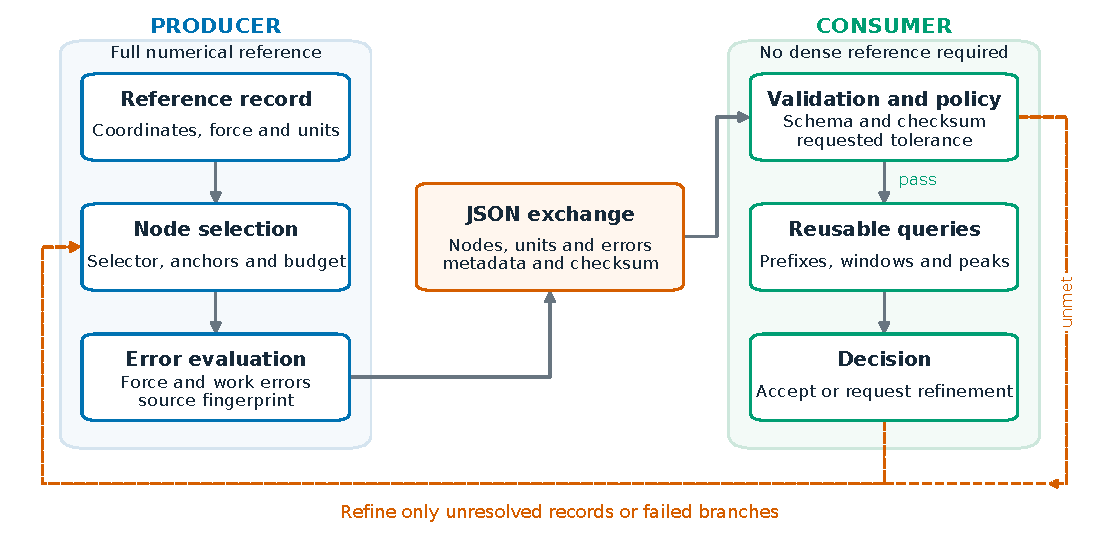
\includegraphics[width=\linewidth]{figures/fig01_architecture.pdf}
\caption{Producer--consumer workflow. Error evaluation uses the full reference at production; subsequent queries use the exchanged table. An application checks tolerance status before accepting results and requests finer source tables when needed. OpenAI Codex assisted with the archived diagram code.}\label{fig:architecture}\end{figure}

\subsection{Software functionalities}
Let $F$ be the supplied piecewise-linear (PL) reference on $[0,U]$ with $n$ source nodes and $\widehat F$ its $K$-node interpolant. With $r=F-\widehat F$ and $D(u)=\int_0^u r(s)\,ds$, define
\begin{align}
\eta&=\int_0^U|r(s)|\,ds,&\xi&=(\eta+|D(U)|)/2,\label{eq:area}\\
E_p&=\max|D|,&E_w&=\max D-\min D,\quad\delta=\max|r|.\label{eq:errors}
\end{align}
All extrema include both endpoints. Since an interval error equals $D(b)-D(a)$, $E_w$ is exactly the one-dimensional discrepancy norm of $r$ extended by zero outside the reference domain \cite{Bouchot2014}. An interval joining the minimum and maximum of $D$ attains this range in absolute value. Thus $E_p\leq E_w\leq\xi\leq\eta$; for positive and negative residual areas $P,N$, $\xi=\max(P,N)$. Source nodes and interior zeros of $r$ locate the continuous extrema.

\begin{table}[!htbp]\small\centering
\caption{Reconstruction quantities for the supplied PL reference. Work has units force $\times$ displacement (J for kN and mm); $\delta$ has force units.}\label{tab:measures}
\begin{tabular}{P{.12\linewidth}P{.30\linewidth}P{.48\linewidth}}\toprule
Measure&Definition&Use\\\midrule
$d$&$D(U)$&Terminal error; branch composition\\
$\eta$&$\int_0^U |r(s)|\,ds$&All intervals; conservative bound\\
$\xi$&$\max(P,N)$&All intervals; signed-area bound\\
$E_p$&$\max|D|$&Queries from the reference origin\\
$E_w$&$\max D-\min D$&Queries over any subinterval\\
$\delta$&$\max|r|$&Force fidelity; peak indicators\\\bottomrule
\end{tabular}\end{table}

These are numerical-reference reconstruction quantities. They exclude floating-point arithmetic error and experimental uncertainty. Source verification requires exact hashes and retained coordinates; nonzero numerical fields allow 16 units in the last place (ULPs), while zero must match zero. This is a consistency check, not outward-rounded arithmetic.

Residuals use local force offsets. A compensated balanced scan accumulates trapezoid terms in $O(n)$ work and storage; \path{math.fsum} supplies the terminal sum. Queries integrate endpoint pieces and cached interior ranges instead of subtracting global prefixes. Cached queries cost $O(\log K)$; severe cancellation triggers direct summation with $O(K)$ worst-case cost. Overflow raises \texttt{ValueError}. Unit labels do not rescale values.

Work-priority refinement follows four steps. First, retain the endpoints and requested absolute, positive or negative force peak. Second, evaluate each active interval's PL chord, absolute residual area $\eta_{ab}$ and largest interior vertical residual. Third, remove the interval with largest $\eta_{ab}$ from a priority queue and insert the source node maximizing $|r|$ there. Fourth, replace that interval by its two children and reevaluate the stopping measure. Ties choose the lowest source index. The split maximizes vertical residual; it does not optimize the reduction in area. Vertical priority uses the same split but ranks intervals by $\delta_{ab}$ instead. Uniform and effective-area VW selectors are also available.

Adaptive intervals store terminal residual work and its extrema $(d,l,h)$, together with area and force deviation. Concatenation gives
\begin{equation}
d=d_A+d_B,\quad l=\min(l_A,d_A+l_B),\quad h=\max(h_A,d_A+h_B).\label{eq:composition}
\end{equation}
After rescanning the new child intervals, updating their balanced-tree summaries costs $O(\log K)$, using $O(K)$ tree storage. Residual rescanning retains $O(nK)$ worst-case work. A final full evaluation checks the selected table. Greedy errors need not decrease after every insertion. VW costs $O(n\log n)$. Relative work tolerances use $|W(U)|$; zero terminal work requires an absolute budget.

\subsection{Sample code snippets}
A producer creates a table with an absolute 1 J interval budget and checks attainment before saving it:
{\small
\begin{verbatim}
from workcert import reduce_response, ReducedResponse
import numpy as np
a = np.loadtxt("data/prepared/PLA_STWC-1.csv",
               delimiter=",", skiprows=1)
t = reduce_response(a[:, 0], a[:, 1], method="work",
    max_points=129, tolerance=1., certificate="window",
    x_unit="mm", force_unit="kN")
if t.metadata["tolerance_met"] is not True:
    raise ValueError("Refine before using this table")
t.save("response.json")
c = ReducedResponse.load("response.json")
energy, error = c.window_work(10., 20.), c.certificate.window
\end{verbatim}
}
The consumer obtains a work interval $[\widehat W-E_w,\widehat W+E_w]$. \path{from_indices} imports externally selected nodes; \path{split_monotone_branches} preserves reversals and zero-work dwell events. Query methods expose results even when a construction budget was unmet; applications must enforce their acceptance policy. Section~\ref{sec:cyclic} provides a checked path example.

\subsection{Verification and AI-assisted implementation}
The released package has 81 analytical and regression tests. Both distributions passed six Windows installations; 15 Linux/macOS/Windows and Python 3.10--3.14 workflow jobs passed. Supplementary S1 separates this release evidence from the additional acceptance-policy tests, measurement checks and independent workbook calculations.

OpenAI Codex assisted research planning, data collection, implementation, analysis, plotting and writing, including \path{software/src/workcert}, \path{validation}, \path{authoring} and the scripts in Supplementary S2. Analytical/rational fixtures and independent scalar integration provide expected values. The contributor-verification record identifies the authors' original checks; new automated checks are reported separately with reproduction commands and dependencies.

\section{Illustrative examples}
\subsection{Decision-focused table exchange}\label{sec:decision}
The PLA+ dataset contains 40 singly tested configurations and two triplicate controls: 42 configurations and 46 specimens \cite{Saber2026,Guler2026}. A 1 J interval budget retains 1520 of 46,000 source nodes. For $W(u)=\int_0^u F(s)\,ds$ at stroke $u$, $EA=W(u)$, $SEA=EA/m$, $MCF=EA/u$ and $CFE=MCF/P(u)$ for prefix peak $P(u)$. After the retained source global peak, CFE intervals are $(\widehat W\pm E_p)/(uP)$; earlier queries combine force bounds and retained anchors with a positive peak lower bound.

All 184 indicator sets contain their dense-reference values. Two three-specimen controls at four strokes give eight descriptive scatter comparisons. Their small samples make SD estimates uncertain; the closest prefix-bound/SD ratio is 0.921. Control-mean intervals average specimen endpoints without a $\sqrt3$ reduction. A $\pm0.05$ g mass-rounding scenario changes SEA by at most 0.310\%.

The consumer initially separates 3345 of 3444 configuration pairs and 103 of 164 adjacent pairs in reference order. At 20 mm, it selects the largest SEA lower bound and all rivals whose upper bound reaches it, identifying configurations 26 and 35 for refinement without consulting the reference ranking. Halving their budgets to 0.5 J retains 1538 nodes overall, a net increase of 18; only two replacement tables totaling 81 nodes are transmitted. At the reported masses, configuration 26 exceeds every competing upper bound by 0.00953 kJ/kg. The subsequent reference comparison gives a 0.02340 kJ/kg best--runner-up gap.

Mass rounding leaves this decision unresolved: with $\pm0.05$ g, even full source curves give a worst-case SEA difference of $-0.00344798$ kJ/kg. Additional curve nodes cannot replace more precise masses. The same exchanged table supports an inverse query: a 20-node STWC-1 representation maps 100 J into $[21.812,22.170]$ mm, containing the reference 22.017 mm. Inversion uses the positive-force 10--40 mm loading interval and represents quasi-static work capacity (Fig.~\ref{fig:workflow}).

\begin{figure}[!htbp]\centering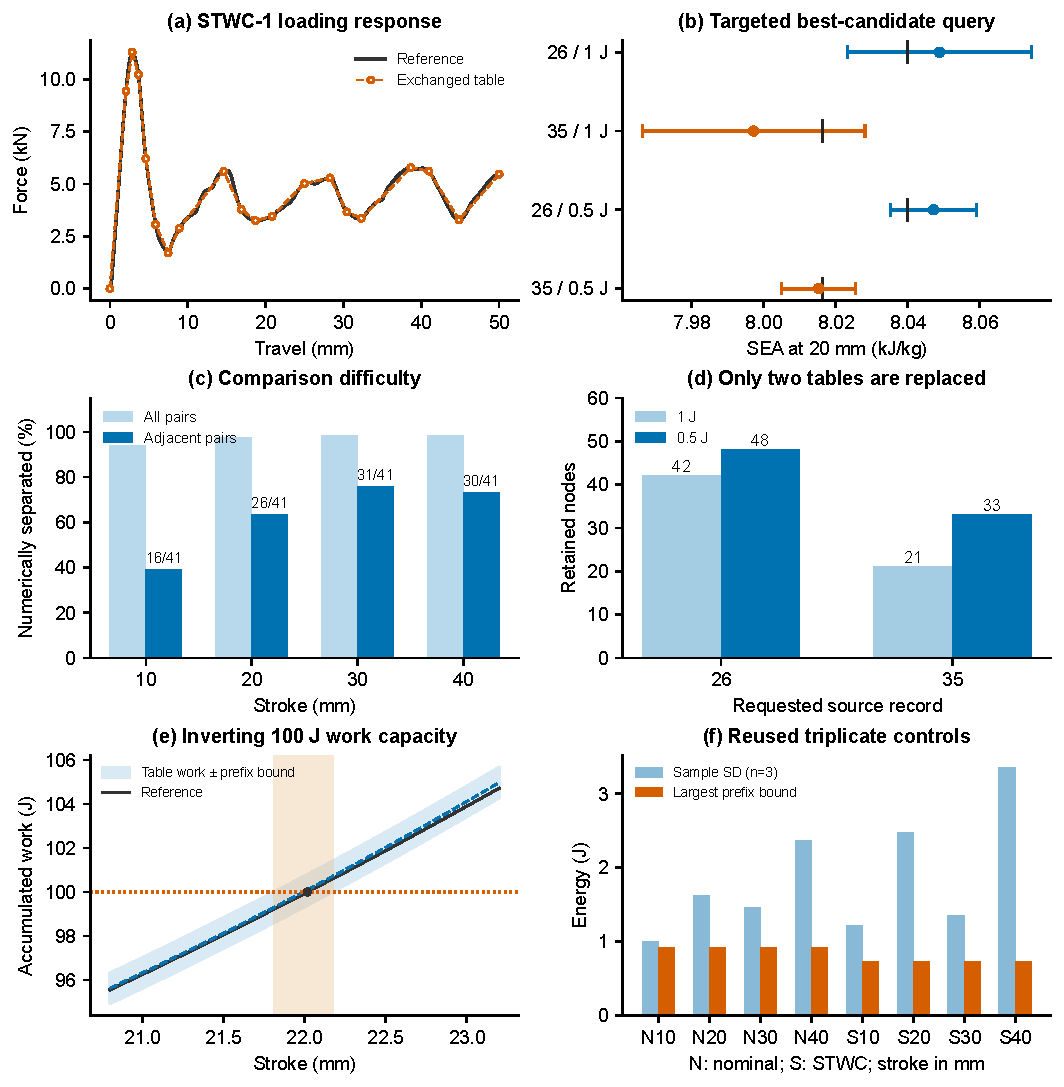
\includegraphics[width=\linewidth]{figures/fig02_decisions.pdf}
\caption{Consumer workflow: reference/table response, candidate intervals at reported masses, adjacent versus all-pair separation, targeted point allocation, inverse work query and repeated-specimen scatter. Reference ticks in (b) are used only for evaluation. OpenAI Codex assisted with the archived plotting code.}\label{fig:workflow}\end{figure}

Workbook checks require published values to lie within the reconstruction intervals, with $10^{-9}$ numerical slack in each indicator's native unit. At reported strokes, EA, SEA, MCF and CFE cover 45/46 entries; peaks cover all 46. Thirteen nominal-50-mm records instead integrate through stored endpoints of 50.004--50.009 mm. Reproducing those endpoints while retaining the reported stroke in the MCF denominator gives 46/46 coverage for every indicator. Independent rational integration leaves maximum differences of $2.73\times10^{-10}$ J for EA and relative differences below $5.8\times10^{-13}$ for the remaining indicators (Supplementary S1).

A separate connector reader verifies a 33-node vertical-priority loading export: $\delta=0.204$ kN, $E_p=0.665$ J and $E_w=0.815$ J. This illustrates force-table exchange; constitutive unloading and solver response require further modeling.

\subsection{Signed cyclic response}\label{sec:cyclic}
A stainless-steel record has 125,157 chronological pairs, 2971 monotone branches and 1984 dwell events \cite{CyclicDataset2024,CyclicPaper2022}. Branch-size quartiles are 2, 9 and 26 nodes. A diagnostic deadband detects 94 reversals, consistent with the 47-cycle S1-L1 record in Table~3 of \cite{CyclicPaper2022}; the integration path is unchanged.

With absolute-peak retention, 129-node caps and branch budgets $0.001|W_b|$, the initial tables retain 13,890 nodes. Branch 2533 has $E_w=0.154223$ J against 0.087194 J requested, so its \path{tolerance_met} flag is false. The checked composer in Supplementary S2 propagates this failed ID to the whole path and rejects budget-qualified use by default. Diagnostic mode retains the failure status. Missing status or an error exceeding its stated budget also prevents acceptance; a failing branch must never be omitted.

Increasing only that branch's cap to 257 yields 153 nodes and $E_w=0.082025$ J. All branch budgets then pass, with 13,914 nodes overall. Source verification precedes recomposition; alternatives are full retention of an unresolved branch or continued rejection, rather than silently relaxing its budget. The recovered path has terminal, prefix and interval errors of 68.488, 68.679 and 68.904 J; summed branch-window bounds give 104.406 J. Acceptance of local budgets does not establish a separately chosen global relative tolerance.

Descending summaries become $(-d,l-d,h-d)$ before Eq.~\eqref{eq:composition}; the reconstruction bounds exclude rounding from sequential float64 composition. The 92.034 kJ reference value is signed chronological work, $\int F\,dx$. A closed quasi-static cycle returning to the same stored-energy state has a loop integral representing hysteretic dissipation, with sign set by convention. This open record runs from $(0\ \mathrm{mm},0\ \mathrm{kN})$ to $(3.1154\ \mathrm{mm},13.0479\ \mathrm{kN})$ and may include stored-energy change; its net work is not a sum of closed-cycle losses.

\begin{figure}[!htbp]\centering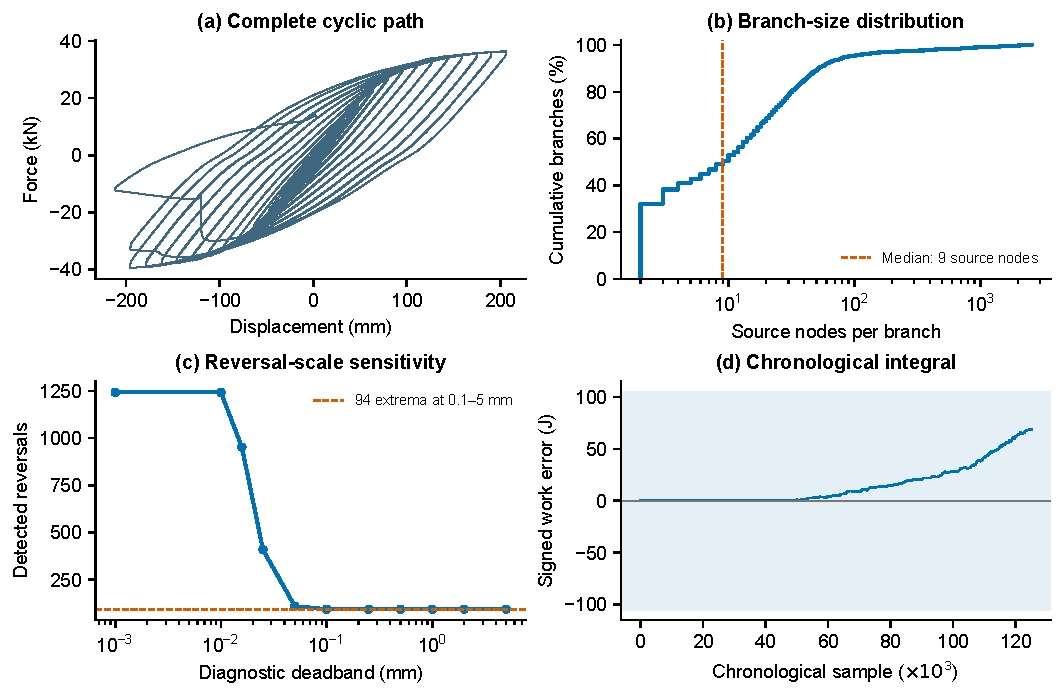
\includegraphics[width=\linewidth]{figures/fig03_cyclic.pdf}
\caption{Initial cyclic representation before targeted recovery: path, branch sizes, reversal diagnostic and chronological work error. Shading shows $\pm\sum_b E_{w,b}$. The checked workflow rejects its one unmet branch budget and refines that branch as described in Section~\ref{sec:cyclic}. OpenAI Codex assisted with the archived plotting code.}\label{fig:cyclic}\end{figure}

\subsection{Selectors and matched-objective controls}\label{sec:selectors}
Comparisons use 23 CX-steel honeycomb records, one enhanced double-arrow honeycomb (EDAH) record and 46 PLA+ curves \cite{Afkhami2022,Afkhami2023,AfkhamiDataset2022,WuDataset2025,Wu2026,Saber2026}. Archived preparation aligns CX contact at 0.5 kN and ends at 40\% of nominal loaded size. Six selectors use 9, 17, 33, 65 and 129 nodes.

The fixed-count RDP baseline scales displacement and force independently to unit range; constant force uses denominator one. It retains the endpoints and first absolute force maximum, then repeatedly splits the chord with greatest perpendicular deviation in normalized coordinates. Thus $K$ includes all anchors. This best-first fixed-count adaptation differs from native tolerance-based RDP, which is checked separately against third-party code (Supplementary S1).

\begin{table}[!htbp]\small\centering
\caption{Median 33-node work errors relative to $|W(U)|$ over 70 references (23 CX, 1 EDAH, 46 PLA+). Ratios use 58 original references with $n\leq1000$: 12 CX and 46 PLA+. Uniform sampling lacks the common peak constraint and is excluded from ratios.}\label{tab:selectors}
\begin{tabular}{lrrrr}\toprule Selector&$E_p$ (\%)&$E_w$ (\%)&$\eta/\eta^*$&$\delta/\delta^*$\\\midrule
Work priority & 0.168 & 0.207 & 1.319 & 2.615 \\
Vertical priority & 0.204 & 0.239 & 1.370 & 1.663 \\
RDP, fixed count & 0.243 & 0.281 & 1.577 & 5.632 \\
Visvalingam--Whyatt & 0.155 & 0.187 & 1.396 & 3.096 \\
Uniform + peak & 0.229 & 0.344 & 2.657 & 10.351 \\
Uniform & 0.231 & 0.364 & -- & -- \\
\bottomrule\end{tabular}\end{table}

VW achieves the lowest pooled median window error (Table~\ref{tab:selectors}), also under equal-cohort and equal-configuration weighting. CX alone favors vertical priority and EDAH favors work priority, although EDAH has only one record. Work priority is therefore an available refinement strategy, not a uniformly best selector (Fig.~\ref{fig:selectors}).

\begin{figure}[!htbp]\centering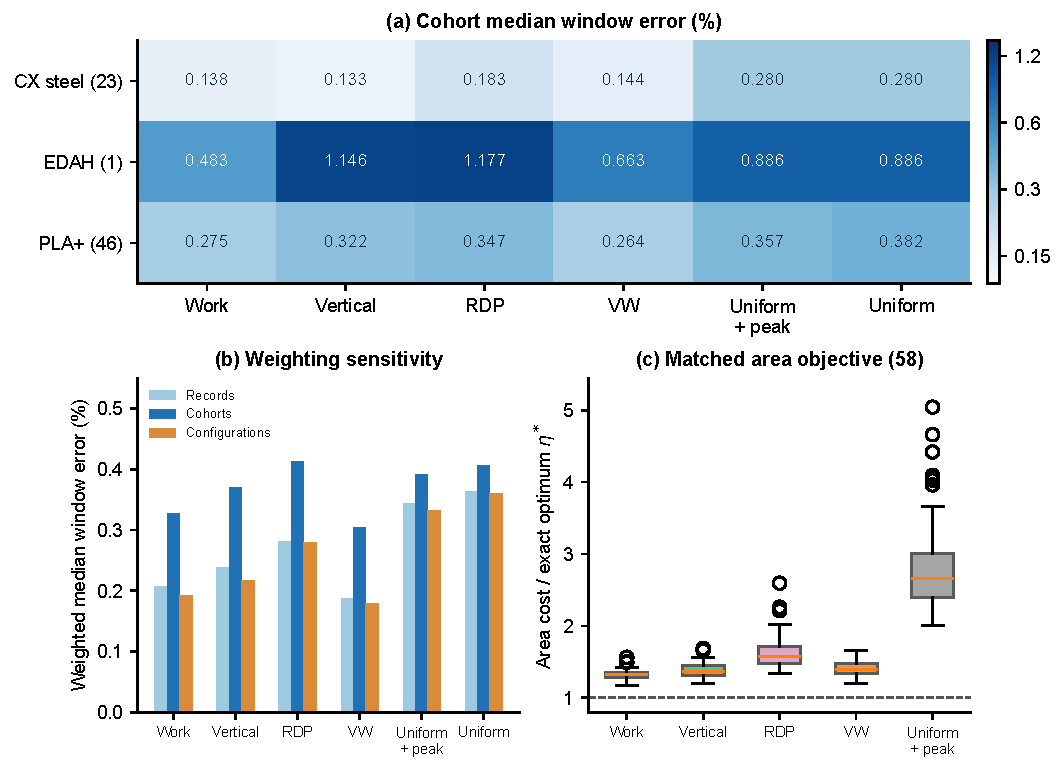
\includegraphics[width=\linewidth]{figures/fig04_selectors.pdf}
\caption{Cohort-specific window errors, weighting sensitivity and matched-area optimality gaps. OpenAI Codex assisted with the archived plotting code.}\label{fig:selectors}\end{figure}

Dynamic programming gives 580 area- or force-optimal paths at the five budgets under identical endpoint and peak constraints. Its $n\leq1000$ ceiling controls the $O(n^3+Kn^2)$ benchmark cost, rather than restricting WorkCert. The 12 larger references are excluded by length, without downsampling. Neither objective establishes prefix- or window-error optimality.

All 70 references enter the 1\% stopping comparison with full reference length as the cap and identical anchors. All 560 selector--measure cases meet tolerance; none are discarded. Within work priority, changing only the all-interval stopping measure from conservative $\eta$ to direct $E_w$ reduces median nodes from 27 to 14. Prefix-only stopping addresses a different requirement.

\subsection{Exchange costs and query performance}\label{sec:exchange}
Actual uncompressed JSON sizes include coordinates, indices, units, error metadata, source fingerprints and payload checksums. Across the 70 references, 33-node work-priority tables have median size 1712.5 bytes, versus 20,401 bytes for full-node tables in the same schema. Compact dense JSON without error metadata, indices or checksum has median size 16,027.5 bytes.

Three independent processes each take five timed repetitions after warm-up, using a warm file cache and 10,000-query batches (Fig.~\ref{fig:scale}). On an Intel Core i5-11300H, 15.69 GiB RAM, Windows 10, Python 3.12.14 and NumPy 2.3.5, median reduced/full-schema loading times are 0.758/3.101 ms. Loading includes validation and integration-cache construction. Compact dense JSON parses in 0.589 ms but supplies neither operation. Reduced/full-schema prefix queries take 2.832/5.106 ms per batch; interval queries take 3.427/5.976 ms. Each value is a median across curves of per-curve process medians.

No direct-summation fallback occurs at the 1.4 million tested prefix/window locations for either representation. A separate cancellation fixture exposes its cost: 256 full-domain queries on 100,001 nodes take 2.278 s with fallback and 0.900 ms in a diagnostic bypass. Fallback returns $2\times10^{-100}$ J; bypass loses that value entirely. This deliberate stress test illustrates the linear-cost accuracy safeguard, not typical compression-query speed.

\begin{figure}[!htbp]\centering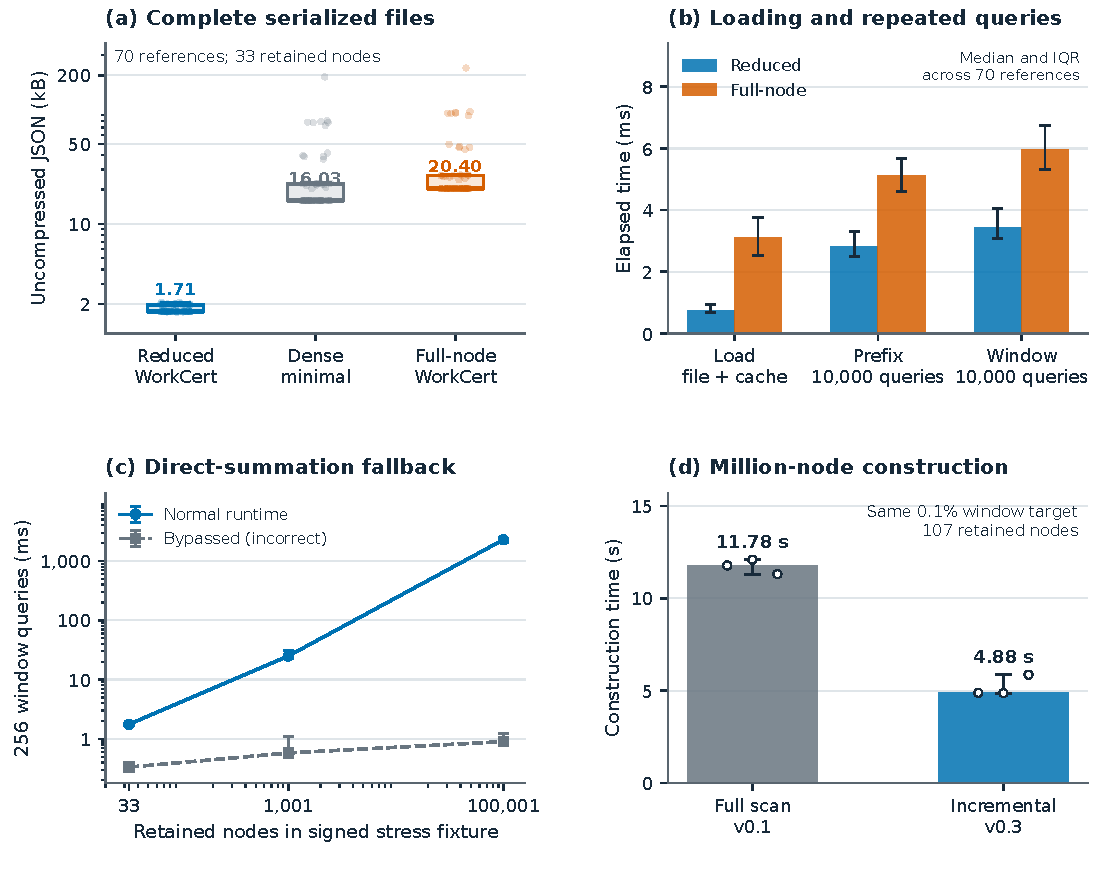
\includegraphics[width=\linewidth]{figures/fig05_exchange_scale.pdf}
\caption{Measured storage and execution costs: (a) serialized size including metadata; (b) loading and repeated queries; (c) cancellation-triggered fallback; (d) construction scaling. Panels (a,b) summarize 70 references; bars and whiskers in (b) show medians and interquartile ranges across curves. Each curve uses three processes and five timed repetitions; panel (c) uses three repetitions per process, with minimum--maximum process ranges. Its bypass returns an incorrect result. Panel (d) shows three-process construction medians and ranges. OpenAI Codex assisted with the archived plotting code.}\label{fig:scale}\end{figure}

At one million synthetic samples and 0.1\% window tolerance, construction takes 11.78 s for full-scan version 0.1 and 4.88 s for stable incremental construction, retaining 107 nodes. Small cases incur tree overhead; Supplementary S1 details the original protocol and precision fixtures.

\section{Impact}
Database curators can exchange a table once and support subsequent work queries with explicit source-relative errors. The candidate example makes the workflow concrete: consumer intervals identify two records for refinement, and replacement tables resolve the reported-mass comparison. The mass scenario then identifies a measurement requirement that extra curve nodes cannot remedy.

Structural analysts can inspect force and work fidelity before using a loading table. Researchers can compare externally selected nodes through the same error and persistence interface. Cyclic-data users can check branch attainment before combining paths. Full source exchange remains practical for these small databases; the main benefit is portable error accounting and selective refinement. Independent laboratory adoption and solver-level effects remain topics for evaluation.

\FloatBarrier
\section{Conclusions}
WorkCert connects source-relative reconstruction errors to reusable queries, selective refinement and checked cyclic composition. Selector choice depends on the objective; VW has the lowest pooled median window error here. The bounds exclude measurement uncertainty and arithmetic rounding. Reproducible scripts preserve both accepted results and unmet-budget diagnostics.
\section*{CRediT authorship contribution statement}
\textbf{Saisai Hou:} Conceptualization, Methodology, Software, Formal analysis, Visualization, Writing -- original draft.
\textbf{Yunzhi Zhu:} Methodology, Validation, Data curation, Writing -- review \& editing.
\textbf{Sen Zhang:} Conceptualization, Supervision, Resources, Writing -- review \& editing, Project administration.
\section*{Declaration of competing interest}
The authors declare no competing interests.
\section*{Funding}
This work was supported by the General Program of Natural Science Research (Basic Science) in Higher Education Institutions of Jiangsu Province (Grant No. 25KJD110002).
\section*{Acknowledgements}
The authors thank the contributors of the public compression and cyclic-loading datasets.
\section*{Data and code availability}
The CC BY 4.0 data are available at \url{https://doi.org/10.17632/8bxkdw4nfw.1}, \url{https://doi.org/10.5281/zenodo.16399749}, \url{https://doi.org/10.17632/v7p6y654ft.4} and \url{https://doi.org/10.5281/zenodo.10829958}. WorkCert 0.3.0 is fixed at \url{https://github.com/changs1723/WorkCert/tree/v0.3.0} and \url{https://doi.org/10.5281/zenodo.23934502}. The original article's complete inputs are fixed at \url{https://github.com/changs1723/WorkCert/tree/article-v0.3.0-final}. Supplementary S1 provides technical notes; Supplementary S2 supplies this revision's scripts, results, manuscript sources and build instructions. They use the fixed original inputs and the unchanged released runtime.
\section*{Declaration of generative AI and AI-assisted technologies in the manuscript preparation process}
OpenAI Codex (OpenAI) assisted with research planning, literature and public-data collection, implementation and debugging, numerical analysis and verification, figure preparation, drafting, language editing and typesetting. The authors are responsible for the research design, interpretation, software, results and final manuscript.
\bibliographystyle{elsarticle-num}{\small\bibliography{references}}
\end{document}
